% !TEX root = main.tex

% Preamble
\documentclass[11pt]{report}
\hbadness=10000

% Load a custom .sty file that includes all required packages
\usepackage{packages} % Replace 'packages.sty' with actual package names if needed

% Package for setting line spacing
\usepackage{setspace}

% Uncomment if acronyms and nomenclature files are used
%\input{acronym} % Load acronyms
%\input{nomencl} % Load nomenclature

% Bibliography setup with BibLaTeX
\addbibresource{refs.bib} % Add bibliography file

% Set page margins
\geometry{
  a4paper,
  left=20mm,
  right=20mm,
  top=15mm,
  bottom=30mm
}

% Remove paragraph indentation
\setlength{\parindent}{0pt}

% Import titlesec package
\usepackage{titlesec}

% Format chapter, section, subsection, and subsubsection headings
\titleformat{\chapter}{\normalfont\huge\bfseries}{\thechapter.}{1em}{}
\titleformat{\section}{\normalfont\Large\bfseries}{\thesection}{1em}{}
\titleformat{\subsection}{\normalfont\large\bfseries}{\thesubsection}{1em}{}
\titleformat{\subsubsection}{\normalfont\normalsize\bfseries}{\thesubsubsection}{1em}{}


% Document content begins
\begin{document}

% Set page numbering to arabic
\pagenumbering{arabic}

% Include the cover page
% Temporarily change geometry for the title page
\newgeometry{
    left=10mm,  % Removes left margin
    right=10mm, % Removes right margin
    top=5mm,   % Removes top margin
    bottom=5mm % Removes bottom margin
}

\begin{titlepage}
    \begin{tikzpicture}[remember picture, overlay]
        % Cover image on the left side of the page
        \node[anchor=north west, inner sep=0] at ([xshift=0mm,yshift=-40mm]current page.north west) {
            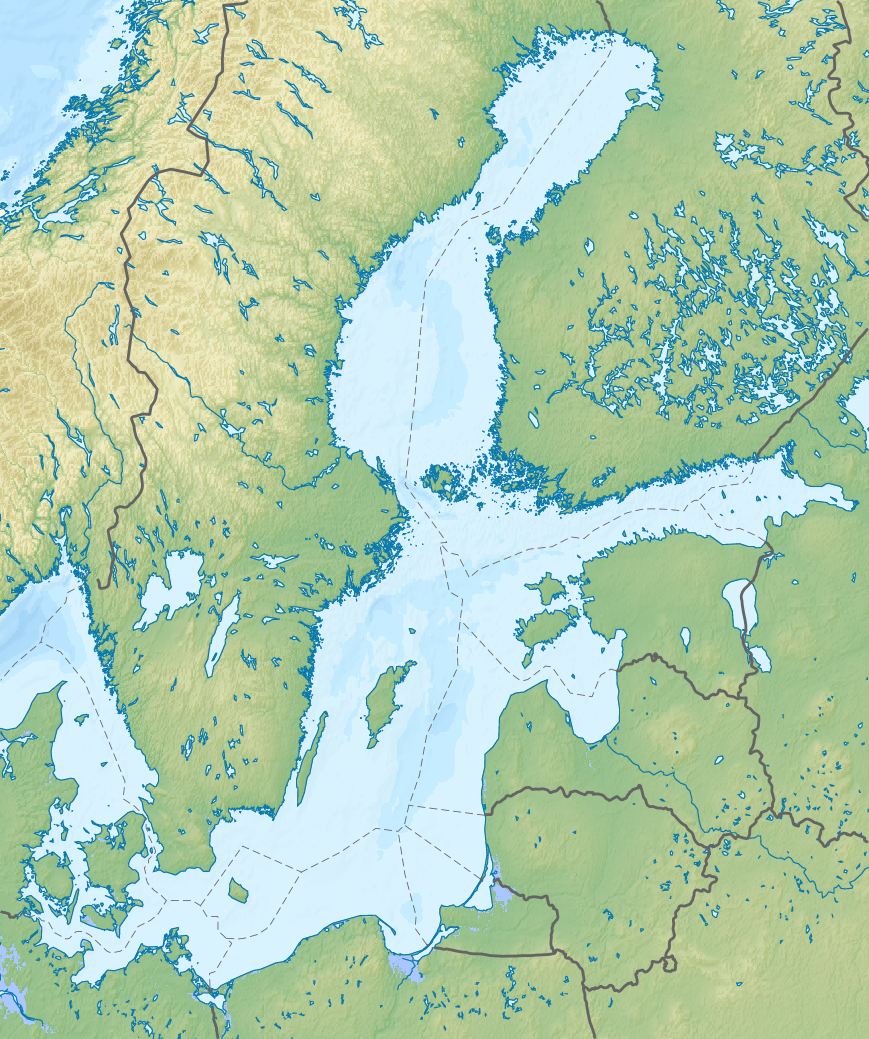
\includegraphics[height=0.7\paperheight,width=.55\paperwidth,keepaspectratio,
            clip,trim=60 0 180 0]{Figure/Cover/Relief_Map_of_Baltic_Sea.png}
        };

        % Logos aligned horizontally on the top left
        \node[anchor=north west, inner sep=10mm] at ([xshift=-5mm,yshift=0mm]current page.north west) {
            \begin{minipage}[t]{0.55\paperwidth}
                \begin{minipage}[c]{0.4\linewidth}
                    
\includegraphics[width=\linewidth]{Figure/Cover/TUDelft_logo_rgb.png}
                \end{minipage}
                \hspace{0.5cm} % Space between the logos
                \begin{minipage}[c]{0.4\linewidth}
                    
\includegraphics[width=\linewidth]{Figure/Cover/logo_wb.png}
                \end{minipage}
            \end{minipage}
        };

        % Thesis title and other information in the middle right
        \node[anchor=center, inner sep=0] at ([xshift=-50mm,yshift=0]current page.east) {
            \begin{minipage}[c]{0.4\paperwidth}
                \begin{spacing}{1.2}
                {\huge Energy System Modelling\par}
                {\huge of the Baltic Sea Region:\par}
                {\huge A Techno-Economic\par}
                {\huge Optimisation of\par}
                {\huge Offshore Wind Farms,\par}
                {\huge Substations, and \par}
                {\huge Electrical Infrastructure \par}
                {\huge for Predicting Future \par}
                {\huge Strategic Development \par}
                \vspace{2cm}
                {\Large\bfseries Constantijn F.L. de Wilt\par}
                \vspace{0.5cm}
                {\Large Master Thesis\par}
                {\Large \today\par}
                \end{spacing}
            \end{minipage}
        };

        % Supervisors and other details at the bottom left
        \node[anchor=south west, inner sep=0] at ([xshift=5mm,yshift=20mm]current page.south west) {
            \begin{minipage}[t]{0.9\textwidth}
                {\setlength{\extrarowheight}{10pt}
                \begin{tabular}{@{}rl@{}}
                    \Large Degree:      & \Large MSc Sustainable Energy Technology \\
                    \Large Supervisors: & \Large Michiel Zaayer (Delft University of Technology)\\
                                        & \Large Marco Plantema (Witteveen+Bos)\\
                \end{tabular}}
            \end{minipage}
        };
    \end{tikzpicture}

    % Clear the rest of the page to prevent overlap
    \null
    \newpage
\end{titlepage}

% Restore the geometry for the rest of the document
\restoregeometry

\newpage

% Include main content chapters
% Uncomment if summary is used
%\input{Main/summary}

% Include chapters from Main directory
%\input{Main/1.1Introduction}
%\input{Main/1.2Objectives}

% \input{Main/2.1Background}
% \input{Main/2.2Calculations}
% \input{Main/2.3Geoprocessing}
\chapter{Modelling}

The objective function aims to minimize the total cost of an energy system configuration by summing up various cost components. It includes expenses related to selected wind farms, operational costs of energy hubs, and expenditures on export cables connecting wind farms to energy hubs and energy hubs to onshore substations. The function iterates over viable options for each component, aggregating their respective costs. By minimizing this total cost, the optimization process seeks an efficient configuration that balances the need for renewable energy generation with cost-effectiveness. \\


To express the objective function in a mathematical equation, you can represent it as the sum of individual costs:

The objective function \( \text{global\_cost\_obj} \) can be represented as:

\begin{equation}
\label{eq:objective_function}
\text{\small \emph{Minimize:} } \sum_{\substack{\text{wind} \\ \text{farms}}} C_{WF} + 
\sum_{\substack{\text{energy} \\ \text{hubs}}} C_{EH} + 
\sum_{\substack{\text{onshore} \\ \text{substations}}} C_{ONSS} +
\sum_{\substack{\text{export} \\ \text{cables 1}}} C_{EC1} + 
\sum_{\substack{\text{export} \\ \text{cables 2}}} C_{EC2}
\end{equation}


Where:
\begin{itemize}
    \item \( \sum_{\substack{\text{wind} \\ \text{farms}}} C_{WF} \) denotes the summation over the total cost of all selected wind farms,
    \item \( \sum_{\substack{\text{energy} \\ \text{hubs}}} C_{EH} \) denotes the summation over the total cost of all selected energy hubs,
    \item \( \sum_{\substack{\text{onshore} \\ \text{substations}}} C_{ONSS} \) denotes the summation over the total cost of all selected onshore substations,
    \item \( \sum_{\substack{\text{export} \\ \text{cables 1}}} C_{EC1} \) denotes the summation over the total cost of export cables connecting wind farms to energy hubs,
    \item \( \sum_{\substack{\text{export} \\ \text{cables 2}}} C_{EC2} \) denotes the summation over the total cost of export cables connecting energy hubs to onshore substations.
\end{itemize}


\section*{Variable Definitions}

\begin{itemize}
    \item \( \text{C}_{\text{WF}}[wf] \): Capacity of wind farm \( wf \)
    \item \( \mathcal{W} \): Set of viable wind farm IDs
    \item \( x_{wf} \): Binary variable indicating whether wind farm \( wf \) is selected
    \item \( \mathcal{H} \): Set of viable energy hub IDs
    \item \( C_{\text{WF-EH}}[wf, eh] \): Connection capacity variable between wind farm \( wf \) and energy hub \( eh \)
    \item \( \mathcal{I}_{\text{WF-EH}} \): Set of viable (wind farm, energy hub) connection IDs
    \item \( C_{\text{EH}}[eh] \): Capacity variable for energy hub \( eh \)
    \item \( \mathcal{I}_{\text{EH-ONSS}} \): Set of viable (energy hub, onshore substation) connection IDs
    \item \( C_{\text{EH-ONSS}}[eh, onss] \): Connection capacity variable between energy hub \( eh \) and onshore substation \( onss \)
    \item \( \mathcal{S} \): Set of viable onshore substation IDs
    \item \( C_{\text{ONSS}}[onss] \): Capacity variable for onshore substation \( onss \)
\end{itemize}

\section*{Constraint Definitions}

\subsection*{Total Capacity Constraint}
Ensure the selected wind farms collectively meet a minimum required capacity.
\begin{equation}
    \sum_{wf \in \mathcal{W}} x_{wf} \cdot \text{C}_{\text{WF}}[wf] \geq \sum_{wf \in \mathcal{W}} \text{C}_{\text{WF}}[wf]
\end{equation}

\subsection*{Capacity Constraints}
\subsubsection*{Connection from Wind Farms to Energy Hubs}
Ensure each selected wind farm is connected to exactly one energy hub, and the connection capacity matches the selected wind farm's capacity.
\begin{equation}
    \sum_{eh \in \mathcal{H}} C_{\text{WF-EH}}[wf, eh] \geq x_{wf} \cdot \text{C}_{\text{WF}}[wf] \quad \forall wf \in \mathcal{W}
\end{equation}

\subsubsection*{Capacity of Energy Hubs}
Ensure the capacity of each energy hub matches or exceeds the total capacity of the connected wind farms.
\begin{equation}
    C_{\text{EH}}[eh] \geq \sum_{wf \in \mathcal{W}} C_{\text{WF-EH}}[wf, eh] \quad \forall eh \in \mathcal{H}
\end{equation}

\subsubsection*{Connection from Energy Hubs to Onshore Substations}
Ensure the connection capacity from each energy hub to onshore substations matches the substation's capacity.
\begin{equation}
    \sum_{onss \in \mathcal{S}} C_{\text{EH-ONSS}}[eh, onss] \geq C_{\text{EH}}[eh] \quad \forall eh \in \mathcal{H}
\end{equation}

\subsubsection*{Capacity of Onshore Substations}
Ensure the capacity of each onshore substation is at least the total incoming capacity from the connected energy hubs.
\begin{equation}
    C_{\text{ONSS}}[onss] \geq \sum_{eh \in \mathcal{H}} C_{\text{EH-ONSS}}[eh, onss] \quad \forall onss \in \mathcal{S}
\end{equation}

\section*{Mathematical Operators}

\begin{itemize}
    \item \( \sum \): Summation operator, which adds up a sequence of numbers.
    \item \( \geq \): Greater than or equal to, ensures the left-hand side is at least as large as the right-hand side.
    \item \( \forall \): For all, used to indicate that the expression applies to all elements of the specified set.
    \item \( \cdot \): Multiplication operator.
\end{itemize}

\section*{Constraint Definitions and Explanations}

\subsection*{1. Total Capacity Constraint}

\textbf{Mathematical Expression:}
\[
\sum_{wf \in \mathcal{W}} x_{wf} \cdot \text{C}_{\text{WF}}[wf] \geq \sum_{wf \in \mathcal{W}} \text{C}_{\text{WF}}[wf]
\]

\textbf{Explanation:}
\begin{itemize}
    \item \textbf{Objective:} Ensure the selected wind farms collectively meet a minimum required capacity.
    \item \textbf{Left-hand Side:} The total capacity of the selected wind farms. This is calculated by summing the capacities of all wind farms \( \text{C}_{\text{WF}}[wf] \) that are selected (\( x_{wf} = 1 \)).
    \item \textbf{Right-hand Side:} The total potential capacity of all considered wind farms.
    \item \textbf{Logic:} The total capacity of the wind farms that are selected should be at least equal to the total potential capacity of all wind farms. This ensures that the selected wind farms meet a minimum capacity requirement.
\end{itemize}

\subsection*{2. Connection from Wind Farms to Energy Hubs}

\textbf{Mathematical Expression:}
\[
\sum_{eh \in \mathcal{H}} C_{\text{WF-EH}}[wf, eh] \geq x_{wf} \cdot \text{C}_{\text{WF}}[wf] \quad \forall wf \in \mathcal{W}
\]

\textbf{Explanation:}
\begin{itemize}
    \item \textbf{Objective:} Ensure each selected wind farm is connected to exactly one energy hub, and the connection capacity matches the selected wind farm's capacity.
    \item \textbf{Left-hand Side:} The total connection capacity between a wind farm \( wf \) and all viable energy hubs.
    \item \textbf{Right-hand Side:} The capacity of the wind farm \( wf \) if it is selected.
    \item \textbf{Logic:} For each wind farm \( wf \) in the set of viable wind farms \( \mathcal{W} \), the total connection capacity to energy hubs should be at least as much as the capacity of the wind farm if it is selected. This ensures that each selected wind farm is appropriately connected to energy hubs.
\end{itemize}

\subsection*{3. Capacity of Energy Hubs}

\textbf{Mathematical Expression:}
\[
C_{\text{EH}}[eh] \geq \sum_{wf \in \mathcal{W}} C_{\text{WF-EH}}[wf, eh] \quad \forall eh \in \mathcal{H}
\]

\textbf{Explanation:}
\begin{itemize}
    \item \textbf{Objective:} Ensure the capacity of each energy hub matches or exceeds the total capacity of the connected wind farms.
    \item \textbf{Left-hand Side:} The capacity of energy hub \( eh \).
    \item \textbf{Right-hand Side:} The total capacity of all wind farms connected to the energy hub \( eh \).
    \item \textbf{Logic:} For each energy hub \( eh \) in the set of viable energy hubs \( \mathcal{H} \), the capacity of the energy hub should be at least as much as the total capacity of the wind farms connected to it. This ensures that the energy hub can handle all incoming power from the connected wind farms.
\end{itemize}

\subsection*{4. Connection from Energy Hubs to Onshore Substations}

\textbf{Mathematical Expression:}
\[
\sum_{onss \in \mathcal{S}} C_{\text{EH-ONSS}}[eh, onss] \geq C_{\text{EH}}[eh] \quad \forall eh \in \mathcal{H}
\]

\textbf{Explanation:}
\begin{itemize}
    \item \textbf{Objective:} Ensure the connection capacity from each energy hub to onshore substations matches the energy hub's capacity.
    \item \textbf{Left-hand Side:} The total connection capacity from energy hub \( eh \) to all viable onshore substations.
    \item \textbf{Right-hand Side:} The capacity of the energy hub \( eh \).
    \item \textbf{Logic:} For each energy hub \( eh \) in the set of viable energy hubs \( \mathcal{H} \), the total connection capacity to onshore substations should be at least as much as the capacity of the energy hub. This ensures that the connection capacity from the energy hub to onshore substations matches the energy hub's capacity.
\end{itemize}

\subsection*{5. Capacity of Onshore Substations}

\textbf{Mathematical Expression:}
\[
C_{\text{ONSS}}[onss] \geq \sum_{eh \in \mathcal{H}} C_{\text{EH-ONSS}}[eh, onss] \quad \forall onss \in \mathcal{S}
\]

\textbf{Explanation:}
\begin{itemize}
    \item \textbf{Objective:} Ensure the capacity of each onshore substation is at least the total incoming capacity from the connected energy hubs.
    \item \textbf{Left-hand Side:} The capacity of onshore substation \( onss \).
    \item \textbf{Right-hand Side:} The total connection capacity from all energy hubs to the onshore substation \( onss \).
    \item \textbf{Logic:} For each onshore substation \( onss \) in the set of viable onshore substations \( \mathcal{S} \), the capacity of the onshore substation should be at least as much as the total incoming capacity from the connected energy hubs. This ensures that the onshore substation can handle all incoming power from the energy hubs.
\end{itemize}

\section*{Variable Definitions}

\begin{itemize}
    \item \( C_{\text{ONSS}}[onss] \): Cost variable for onshore substation \( onss \)
    \item \( E_{\text{ONSS}}[onss] \): Calculated cost for onshore substation \( onss \)
    \item \( \mathcal{S} \): Set of viable onshore substation IDs
\end{itemize}

\section*{Constraint Definition and Explanation}

\subsection*{Cost Constraint for Onshore Substations}

\textbf{Mathematical Expression:}
\[
C_{\text{ONSS}}[onss] \geq E_{\text{ONSS}}[onss] \quad \forall onss \in \mathcal{S}
\]

\textbf{Explanation:}
\begin{itemize}
    \item \textbf{Objective:} Ensure the cost variable for each onshore substation meets or exceeds the calculated cost.
    \item \textbf{Left-hand Side:} The cost variable for onshore substation \( onss \).
    \item \textbf{Right-hand Side:} The calculated cost for onshore substation \( onss \).
    \item \textbf{Logic:} For each onshore substation \( onss \) in the set of viable onshore substations \( \mathcal{S} \), the cost variable should be at least as much as the calculated cost. This ensures that the cost assigned to each onshore substation is sufficient to cover the calculated cost.
\end{itemize}


\section*{Variable Definitions}

\begin{itemize}
    \item \( \mathcal{W} \): Set of viable wind farm IDs
    \item \( \mathcal{H} \): Set of viable energy hub IDs
    \item \( \mathcal{S} \): Set of viable onshore substation IDs
    \item \( \mathcal{I}_{\text{WF-EH}} \): Set of viable (wind farm, energy hub) connection IDs
    \item \( \mathcal{I}_{\text{EH-ONSS}} \): Set of viable (energy hub, onshore substation) connection IDs
    \item \( \text{Cost}_{\text{WF}}[wf] \): Cost of wind farm \( wf \)
    \item \( \text{Cost}_{\text{EH}}[eh] \): Cost of energy hub \( eh \)
    \item \( \text{Cost}_{\text{ONSS}}[onss] \): Cost variable for onshore substation \( onss \)
    \item \( \text{Cost}_{\text{WF-EH}}[wf, eh] \): Cost of connection between wind farm \( wf \) and energy hub \( eh \)
    \item \( \text{Cost}_{\text{EH-ONSS}}[eh, onss] \): Cost of connection between energy hub \( eh \) and onshore substation \( onss \)
\end{itemize}

\section*{Objective Function}

\textbf{Mathematical Expression:}
\[
\begin{aligned}
\text{\emph{Minimize} } & 
\quad \sum_{wf \in \mathcal{W}} \text{Cost}_{\text{WF}}[wf] + 
\sum_{eh \in \mathcal{H}} \text{Cost}_{\text{EH}}[eh] + 
\sum_{onss \in \mathcal{S}} \text{Cost}_{\text{ONSS}}[onss] \\
& + \sum_{(wf, eh) \in \mathcal{I}_{\text{WF-EH}}} \text{Cost}_{\text{WF-EH}}[wf, eh] + 
\sum_{(eh, onss) \in \mathcal{I}_{\text{EH-ONSS}}} \text{Cost}_{\text{EH-ONSS}}[eh, onss]
\end{aligned}
\]

\textbf{Explanation:}
\begin{itemize}
    \item \textbf{Objective:} Minimize the total cost of the energy system.
    \item \textbf{Components of the Total Cost:}
    \begin{itemize}
        \item \( \sum_{wf \in \mathcal{W}} \text{Cost}_{\text{WF}}[wf] \): The total cost of selected wind farms.
        \item \( \sum_{eh \in \mathcal{H}} \text{Cost}_{\text{EH}}[eh] \): The operational cost of selected energy hubs.
        \item \( \sum_{onss \in \mathcal{S}} \text{Cost}_{\text{ONSS}}[onss] \): The cost variable for onshore substations.
        \item \( \sum_{(wf, eh) \in \mathcal{I}_{\text{WF-EH}}} \text{Cost}_{\text{WF-EH}}[wf, eh] \): The cost associated with export cables connecting wind farms to energy hubs.
        \item \( \sum_{(eh, onss) \in \mathcal{I}_{\text{EH-ONSS}}} \text{Cost}_{\text{EH-ONSS}}[eh, onss] \): The cost associated with export cables connecting energy hubs to onshore substations.
    \end{itemize}
\end{itemize}


\section*{Variable Definitions}

\begin{table}[h!]
\centering
\begin{tabular}{|>{\centering\arraybackslash}m{3cm}|>{\centering\arraybackslash}m{10cm}|}
\hline
\textbf{Variable} & \textbf{Definition} \\
\hline
\( \mathcal{W} \) & Set of viable wind farm IDs \\
\hline
\( \mathcal{H} \) & Set of viable energy hub IDs \\
\hline
\( \mathcal{S} \) & Set of viable onshore substation IDs \\
\hline
\( \mathcal{I}_{\text{WF-EH}} \) & Set of viable (wind farm, energy hub) connection IDs \\
\hline
\( \mathcal{I}_{\text{EH-ONSS}} \) & Set of viable (energy hub, onshore substation) connection IDs \\
\hline
\( \text{C}_{\text{WF}}[wf] \) & Capacity of wind farm \( wf \) \\
\hline
\( x_{wf} \) & Binary variable indicating whether wind farm \( wf \) is selected \\
\hline
\( C_{\text{WF-EH}}[wf, eh] \) & Connection capacity variable between wind farm \( wf \) and energy hub \( eh \) \\
\hline
\( C_{\text{EH}}[eh] \) & Capacity variable for energy hub \( eh \) \\
\hline
\( C_{\text{EH-ONSS}}[eh, onss] \) & Connection capacity variable between energy hub \( eh \) and onshore substation \( onss \) \\
\hline
\( C_{\text{ONSS}}[onss] \) & Capacity variable for onshore substation \( onss \) \\
\hline
\( E_{\text{ONSS}}[onss] \) & Calculated cost for onshore substation \( onss \) \\
\hline
\( \text{Cost}_{\text{WF}}[wf] \) & Cost of wind farm \( wf \) \\
\hline
\( \text{Cost}_{\text{EH}}[eh] \) & Cost of energy hub \( eh \) \\
\hline
\( \text{Cost}_{\text{ONSS}}[onss] \) & Cost variable for onshore substation \( onss \) \\
\hline
\( \text{Cost}_{\text{WF-EH}}[wf, eh] \) & Cost of connection between wind farm \( wf \) and energy hub \( eh \) \\
\hline
\( \text{Cost}_{\text{EH-ONSS}}[eh, onss] \) & Cost of connection between energy hub \( eh \) and onshore substation \( onss \) \\
\hline
\end{tabular}
\caption{Variable Definitions}
\label{tab:variable_definitions}
\end{table}
% \input{Main/2.5Casestudies}

% \input{Main/3.1Conclusion}
% \input{Main/3.2Discussion}



% New page and reset page numbering for bibliography
\newpage
\pagenumbering{gobble} % Removes page numbers

% Include all references regardless of whether they were cited
%\nocite{*}
%\printbibliography[heading=bibintoc, title={Bibliography}]

% End of document content
\end{document}
